\chapter{Probability}
\label{c:probability}

In this chapter we will start thinking about decisions in the context of uncertainty.  Before we get to the {\it decisions} part, we need to talk about the {\it uncertainty} part.

At the outset the idea of uncertainty is pretty straightforward. We often (perhaps always) confront circumstances where we don't know what exactly are the consequences of our actions. Mandy doesn't know whether or not the bus will be on time, but when she leaves her house she must decide whether to walk to the bus stop or hop on her bike. Examples abound.

Academics who study decisions love to discuss gambling devices because of their simplicity.  Dice, coins, and roulette wheels are easy to understand.  Much of the theory of probability was developed initially to deal with games of chance, so it's no surprise it works so well in these contexts.

A dice has six sides, and we have an intuitive idea that each side is equally likely to come up.  This leads to a relatively straightforward way of thinking about our uncertainty.  Our degree of uncertainty in getting a \dice{1} is the same as the degree of uncertainty in getting a \dice{6}.  We are more certain that we will get an even number than than a \dice{3}.  Etc.

\nomenclature{\dice{1}}{To denote the outcome from rolling a 6-sided dice and getting a one (similar for other numbers)}

The central question we will tackle in this chapter is: to what extent should all decisions look like easy cases of dice? Do what extent do people use the same underlying mathematical theory to make all decisions under uncertainty? Regardless of what they actually do, to what extent {\it should} they?

\section{Basic probability}

The theory of probability can become quite complex, especially when one is dealing with situations where there is an infinite number of possibilities.  To keep our lives simple, for the purposes of this chapter, we will always use examples where there are only a finite number of possible outcomes.  This simplifies the theory massively, and will be sufficient for our purposed in this book.

\subsection{Universe of possibility}

We will begin by supposing we have a fixed, finite set of primitive events.  Starting with the dice, this is often represented as the number of pips that come up on the dice.  The primitive set is often represented by the letter $\Omega$, and so in the case of the dice we assume that $\Omega = \{$\dice{1}, \dice{2}, \dice{3}, \dice{4}, \dice{5}, \dice{6}$\}$.  

It is important that we get $\Omega$ right.  We must include everything our agent thinks, for whatever reason, is possible. Maybe they think that the dice could land perfectly on its side or corner, or that the dice turns into a penguin, or whatever.  If they think it's possible, we must include it.  If you are like most of us, you would regard the set $\Omega = \{$\dice{1}, \dice{2}, \dice{5}$\}$ as failing this condition.  This condition is described more formally as saying $\Omega$ is {\it exhaustive}. There is nothing that the agent thinks might occur which is not covered by one of the options in $\Omega$.  

In addition, we must be sure that every item in $\Omega$ is {\it mutually exclusive} with every other item in $\Omega$.  That is, only one option can occur.  With our dice that is covered by the fact that the dice cannot land on more than one side.  We could create a different $\Omega$, which was $\{$Odd, Even$\}$---that is also exhaustive and mutually exclusive.  But we could {\it not} create an $\Omega$ that is $\{$\dice{1}, \dice{2}, \dice{3}, Even, Odd$\}$  While this is exhaustive, it is not mutually exclusive.

For most of our simple illustrative examples, creating $\Omega$ will be relatively easy.  In realistic settings it can sometimes be very complicated, and one can accidentally include too much or too little or some combination thereof.

Returning to our dice example, take the natural $\Omega = \{$\dice{1}, \dice{2}, \dice{3}, \dice{4}, \dice{5}, \dice{6}$\}$.  Now we might want to ask, what about those other things we talked about like the dice coming up even? Or odd? Or less than 6? Or whatever.

To handle these, we will construct {\it events}.  An event is a subset of $\Omega$, which represents some possible set of atomic events that might come about.  The event ``even'' is the set $\{$\dice{2},\dice{4},\dice{6}$\}$, odd is $\{$\dice{1},\dice{3},\dice{5}$\}$, less than six is $\{$\dice{1}, \dice{2}, \dice{3}, \dice{4}, \dice{5}$\}$, etc.  

Since we are restricting ourselves to finitely large $\Omega$'s, we will always consider the space of possible events as the powerset of $\Omega$, $\mathscr{P}(\Omega)$. This gives us a large number of possible events, as many as we might like.  Often this is more than we need, and in infinite settings it can be too much, but for our purposes it will work just fine.

\subsection{Probability}

The basic idea is to represent something like uncertainty or degree of possibility or something like that (more on exactly what we were doing in section~\ref{s:prob-interpretation}).  So a natural first step might be to try and represent this with a number.

If we just left it there, we might end up with some very strange assignments of numbers.  For example, someone might say that it is more likely that they will see a \dice{1} than an odd number. That seems quite strange.

\marginnote{These axioms are often called the Kolmogorov axioms after their inventor \fullcite{ kolmogorov1950}. Of course, various notions of proability have been around much longer.}

So we might want to introduce some constraints, and these are the axioms of probability. We will conjecture a function, $P$, that assigns a number to each event in $\mathscr{P}(\Omega)$.  And then we might ask, what constraints should there be on $P$.  The classic answer is the three axioms of probability:

\nomenclature{$P$}{A probability function}

\begin{enumerate}
\item {\it Normalization}: $P: \mathscr{P}(\Omega) \to [0,1]$
\item {\it Unitarity}: $P(\Omega) = 1$
\item {\it Finite additivty}: $P(E \cup F) = P(E) + P(F)$ when $E$ and $F$ are mutually exclusive
\end{enumerate}

\nomenclature{$[]$}{Used to denote a closed interval of numbers. For example, $[0,1]$ indicates the set of real numbers that are between 0 and 1, inclusive of 0 and 1.}
\nomenclature{+}{Used for numerical addition. Importantly distinct from $\oplus$}
\nomenclature{=}{Used for identity. Importantly distinct from $\sim$.}
\nomenclature{$\cup$}{Set theoretic union. $X \cup Y$ represents the set that has all the members of $X$ and all the members of $Y$ together in one set.}

The first axiom tells us what numbers to use.  We will not have any negative probabilities or probabilities higher than 1.  Why that set?  Well\dots there are many answers.  We will come back to that question in a minute, but for the moment please just go with me on that.  One simple answer to the question is, why not? We can map any other closed set of numbers into that one, and it's convenient for other reasons. 

The second axiom just requires that the universe of all possibilities be assigned probability 1.  That enforces that the number 1 is the maximum number (not some lower number).

The axiom that really does work is finite additivity.  It asserts that if you have two events that have no atomic events in common, the probability of one or the other event is equal to  the sum of the probability of each of the events.\marginnote{A brief note on infinity: If we were dealing with infinite $\Omega$, then we {\it might} want to expand finite additivity to include countable collections of mutually exclusive events.  But maybe not, there is a debate.  Since we are keeping our feet firmly planted in the finite, we won't worry about that any more here.}

\subsection{Expectation}

Although it can seem very simple, with just these three little axioms, probability theory does a lot.  Basically all of statistics is built on top of these axioms. It underpins, science, finance, and much else.

Of course, we won't dive into many of the details here, but we do want to highlight one concept that will become important in later chapters, and that's called {\it expectation}.  

We begin by assigning a numerical value to each individual atomic event in $\Omega$.  This numerical value is completely arbitrary, it could represent anything.  It could be how much money I would expect to win on some gamble. It could be how large a tree will grow in different environmental circumstances. It could be how many people would die from the flu given different scenarios for a flu season.  Whatever it is, it's a number that we care about for some reason or another.  This assignment of numbers is called a {\it random variable}.

For concreteness, let's use the dice example and assign a number to each outcome that equals the number of pips on the dice.  So \dice{1} is assigned the number `1,' \dice{2} is assigned `2,' etc.  That's our random variable.

With the random variable in hand, we can ask what is the average or expected value of that random variable.  In the case of the dice we get that by multiplying the value of the variable by the probability of all the states where we get that number.  So, the value is:
\begin{equation*}
    \frac{1}{6} (1) + \frac{1}{6} (2) + \frac{1}{6} (3) + \frac{1}{6} (4) + \frac{1}{6} (5) + \frac{1}{6} (6) = 3.5
\end{equation*}

This number immediately shows how the word ``expectation'' is a bit strange here.  Do you expect the dice to come up 3.5?  No, of course not. It's impossible to get a 3.5 on a dice. What the mathematical expectation represents is an average. If you rolled the dice many times, on average the value of the variable would be 3.5

When the random variable is a utility, then we call this the expected utility of a decision.  But, we're getting ahead of ourselves.  Without a more sophisticated notion of utility, we can't do that with utilities yet. (Do you remember why?)  We'll come back to this in chapter~\ref{c:vnm}.

\section{What does probability mean?}
\label{s:prob-interpretation}

We laid down a commonly used series of axioms.  But just because something is commonly used doesn't mean its the right thing to do.  Why should we use these axioms rather than some other?  What about these axioms makes them the correct way to think about uncertainty.

There are several different answers to this question, and they turn on an even more thorny philosophical question: what does probability mean? So far we've been somewhat cagey about what is the meaning of these numbers.  We've just assigned numbers to events and said they represent something like the degree of uncertainty or the degree of possibility or something like that.

Part of the reason that I've been cagey so far, is that there are several different interpretations of what these numbers represent. Sometimes individual scholars will be confused in their own minds about what they mean, or might mean several things at once, which makes life even harder.  While there are many different interpretations of what probabilities mean, here I would like to present you with some of the most popular.

To make this concrete, let's imagine a very particular probability assignment.  Suppose you have an ordinary 6-sided dice and you say the following sentence ($S$): ``I think the probability that a \dice{1} will appear is $1/6$.''  What does that mean?

Once we have that on the table for each of the interpretations, we can then ask the question: why these axioms rather than some other?

\subsection{Objective chance}

On the {\it objective chance} view, your statement $S$ is saying something about the dice or, more exactly, about the physical system that involves throwing the dice.  You are saying that the dice is not weighted in any way, that the person throwing is not physically capable of influencing the outcome of the side, etc.  

Under this interpretation, the probability of the dice coming up \dice{1} is something like a physical fact in the world.  It is akin to saying that the dice weighs 4.1 grams or that it is made of a type of plastic. It is a claim that is either true or false of the dice and could, in theory, be verified by some type of experiment.

Importantly (to distinguish this from the next interpretation) it is not a statement about many different throws of this dice or about many different similarly constructed dice.  It is a physical statement about this one throw of this one particular dice.  One might come to learn about that physical property from throwing the dice many times, but the physical fact is true regardless of how many times the dice is thrown.

Under this interpretation, what is the justification for the axioms?  Let's consider each in turn.

{\it Normalization}.  This axiom is just a specification of a scale.  We are presuming (perhaps with some additional interpretation) that there is an upper and lower bound to this physical property called ``chance.''  Once we've done that, we can put it on any scale we like, so why not $[0,1]$?  It has some nice mathematical properties that are convenient, and it works just as well as any other.

{\it Unitarity}.  Similarly, this axiom is mostly a convention.  We are specifying that the event that always has the largest of this thing we call ``chance'' is $\Omega$. That does entail {\it some} physical assumptions, but those are in common with the next axiom.

{\it Finite additivity}.  Under the objective chance interpretation, the finite additivity axiom functions something like a law of nature.  (Think, for example, of Newton's law of gravitation.)  It is an empirical fact about how these things, {\it objective chances} behave in the world that might be true or might be false.

It may seem like finite additivity is obvious, but under this interpretation it is not. Not everything in nature adds like this.  Take salt and water.  If you dissolve a particular volume of salt into a volume of water, the resulting salt water will have slightly lower volume than the volume of salt plus the volume of water.  That is, $V($salt$) + V($water$) > V($salt + water$)$. Finite additivity is {\it not} true about the physical property called ``volume.''  Maybe objective chance is like salt and water, the chance of one of two events happening is less than the chance of each added together. Or maybe the addition of two chances leads to more chance than the sum? Or something else entirely.  This is a question for physicists to figure out, once we explain to them what objective chances are.  

\subsection{Relative frequency}

A related, and often conflated, interpretation of probability is the ``relative frequency'' interpretation of probability.  Rather than attributing an objective, physical fact to the claim $S$, the relative frequency interpretation reinterprets this claim to about about many throws of the dice.

The simplest version of relative frequency goes like this: $S$ means ``over the entire history of throws of this dice, \dice{1} will come up exactly 1/6 of the time.''  

You might immediately recognize a problem with this interpretation. What if I buy a brand new dice, never before thrown, and throw it only once?  It comes up \dice{2}. After that I melt the dice down, making sure to never throw it again.

Does that mean that $S$ was false?  That I should have said that the probability of \dice{2} was 1, and the probability of any other number was 0?  That seems strange.  

This is especially troubling for any time that we want to ascribe a probability for an event that might only occur once. What's the probability that the Steelers are going to win the Superbowl in, say, 2050? It's either 1 or 0, because it will only ever happen in 2050 once.

Another version of this interpretation expands the notion of relative frequency beyond just throws of {\it this} dice and includes throws of other relevantly similar dice.  In my hypothetical example of melting down the dice, we might ask what was the frequency of all dice of that form, from that manufacturer?  This would allow us to include many different throws of similar dice.

While this interpretation solves one problem, it also introduces another: what counts as ``similar?''  Known as the {\it reference class} problem, it bedevils actuarial inference.

Suppose that you are a car insurance company and you want to infer what is the probability that I, Kevin Zollman, will get into a car accident this year.  (This is critical for an insurance company, because it needs to decide how much to charge me for insurance.) This event is like the single throw of a dice, it will not be repeated.  Notice, while there are many years where I might get into a car accident, they are not the same. I'm getting older, I might buy different cars, I might drive a longer or shorter distance to work, etc.  

So the insurance company might say the probability is defined by averaging over all drivers in the world; or all of them in the US; or all of the ones in the US who are my age; or all of them who are my age, income, and occupation; or \dots

Each of these will plausibly give you very different answers.  As you define the class more narrowly, you have fewer and fewer examples until you define it so narrowly that you are only left with me. And now you are back to the problem with which we started.

This isn't to say there is no hope for this approach to probability. It does however replace one problem---what is the probability of an event?---with a different problem---what is the appropriate reference class for that event?  I will leave it to you whether the latter problem is any easier than the first.

The more serious concern is that whatever answer you give to the second question will be, in some sense, subjective.  That is, do you think the appropriate reference class for me getting in a car accident includes people of different incomes than me? What about people of different races? Sexes? Ages? Who drive different cars? Who live in different cities? Etc.

To an extent this is a choice based on other beliefs you have. Do you think the chance of a car accident depends on which neighborhood in Pittsburgh you live in?  That's okay, but it does remove some of the appearance of objectivity that many find attractive in the relative frequency interpretation.  Two people might disagree about what is the correct reference class, and therefore what is the correct probability.  What started out seeming quite objective (a relative frequency) has become somewhat more subjective.

What shall we make of the axioms under this interpretation?  For the relative frequency interpretation life is easy. Each of the axioms is just a fact about fractions.  Any relative frequency will be of the form $x/y$ where $x\geq 0$ and $x\leq y$.  So, {\it Normalization} is guaranteed (except perhaps when $x=y=0$).

So long as we specified $\Omega$ correctly, the relative frequency of {\it something} in $\Omega$ happening will be $x/x$.  Something always happens.  So {\it Unitarity} holds. 

The last axiom also follows from basic rules of addition and division.  If a dice was rolled $y$ times and came up \dice{1} $x_1$ times and \dice{2} $x_2$ times, then the relative frequency of it coming up \dice{1} or \dice{2} is given by: $\frac{x_1+x_2}{y}$. So {\it finite additivity} also holds.

\subsection{Degree of belief (subjective Bayesianism)}

The last interpretation of probability that we will discuss is called ``degrees of belief'' or ``subjective Bayesianism.''  The basic idea of this interpretation is that a probability represents some kind of strength or degree of belief: it is a subjective judgment of a single individual.

Because it's subjective, there is no outright fact of the matter.  Two people might differ in their degree of belief that, say, the Steelers will win the Superbowl.  While they might try to provide evidence to convince the other to change their mind, at base we cannot say that one person is right and the other wrong. These are just their degrees of belief.

This fact is often regarded as a problem for this interpretation.  We have a strong intuition that the {\it correct} degree of belief in a \dice{1} coming up on a particular dice is 1/6, and anyone who believes otherwise is {\it wrong}.  Under this interpretation we cannot make sense of this claim.  As we've seen in the previous two interpretations, making that claim precise is somewhat tricky and many think impossible. Because of this, many people (in some cases begrudgingly) accept the subjective interpretation.  

If a probability is just a subjective state, the question about the axioms become particularly pressing.  Why should I obey any of the axioms in my subjective states?  They are my subjective states after all, who are you to tell me how they must behave?  

\section{Qualitative probability}

If we take a subjectivist stance on probably, we treat probability judgments as (mere) reports of subjective states. How confident is Mandy that a \dice{1} will come up on the next roll of the die?  She might be very confident or she might be unsure.  That's entirely up to her.

A critical question then is why should her confidence judgments look anything like a probability?  There are basically two questions one might ask: why should her confidence judgments look anything like numbers at all?  As we found in the last chapter, assigning numbers to judgments like ``Mandy prefers pizza to pasta'' is a tricky business.  There is no guarantee that her judgments will be amenable to assigning numbers.  We might worry about the same thing when it comes to ``Mandy is more confident that a \dice{1} will come up than we will contact intelligent alien life''

Even if we suppose that we could assign numbers to her judgments, there is a further question: why should those numbers obey the axioms of probability? Why can't Mandy's judgments violate one (or more) of the three axioms we laid out?  

There are two broad strategies for answering these questions. The first strategy involves repeating what we did with preference.  Recall that in the chapter~\ref{c:certainty} we started with a qualitative relationship $\succsim$ between two objects: in that case it was something Mandy might receive.  If Mandy obeyed the right set of axioms, then we could turn that qualitative relationship into a quantitative utility function.

Perhaps we could do the same with probability. Maybe we could ask people to rank order events in terms of their likelihood judgments.  We could ask them: do you think it's more likely that we will contact alien life or that a Democrat will be elected US President in 2044?  Once we have those we could convert them into a quantitative probability.  And then (maybe) we can state the probability axioms in a way that makes them seem very intuitive and reasonable.

Although it might be tempting to do things exactly like we did them in the last chapter, we have to be careful.  Ordinary language events can always be added together or broken down.  While  the event ``A Democrat is elected US President in 2044'' seems simple enough, it's actually very complicated. What about ``A Democrat from Pennsylvania is elected in 2044'' or ``A woman Democrat from Pennsylvania is elected in 2044'' etc.

So, when we are asking people to give relative judgments, we have to remember that we are asking them to rank all the events in $\mathscr{P}(\Omega)$ not just the atomic events in $\Omega$. This means that our axioms must be a little more complicated.

Let's get started.  Suppose that we have a set of atomic events $\Omega$ and we want to define a relation ``more likely than'' on all the events in $\mathscr{P}(\Omega)$.  We will use the symbol $\triangleright$ for ``more likely than.''  On first reflection it seems reasonable to insist on the same conditions we had before on $\triangleright$.

\nomenclature{$\triangleright$}{More likely than. $E \triangleright F$ is read as $E$ is more likely than $F$}

\begin{itemize}
    \item $\triangleright$ is irreflexive: it is never the case that $E \triangleright E$ 
    \item $\triangleright$ is asymmetric: If $E \triangleright F$ then $F \cancel{\triangleright} E$.  
    \item $\triangleright$ is transitive: If $E \triangleright F$ and $F \triangleright G$, then $E \triangleright G$
\end{itemize}

\nomenclature{$\cancel{\triangleright}$}{Not more likely than. $E \cancel{\triangleright} F$ is read as $E$ is {\it not} more likely than $F$}

\nomenclature{$E, F, G$}{Arbitrary events, that is subsets of $\Omega$.}

Each of these probably seem quite reasonable for judgements of ``more likely than.''   We can also do the same with ``equally likely as'', which we will represent with $\bowtie$. It will also look similar as before, we will assume that it is reflexive, symmetric, and transitive.  Finally, we will also assume the same three joint conditions on the two, that they are jointly complete, jointly transitive, and strict.

\nomenclature{$\bowtie$}{Equally likely as. $E \bowtie F$ is read as $E$ is equally likely as $F$.}

While the conditions are the same, the interpretations are different.  They may be more or less plausible, and you should take a moment to think through whether you like them or not.  Just like with preference, we could also have started with a weaker relation $\underline\triangleright$ (interpreted as ``at least as likely as'') and defined things that way.  

\nomenclature{$\underline\triangleright$}{At least as likely as.  $E \underline\triangleright F$ is read as $E$ is at least as likely as $F$}

For ordinal utility that is all we needed to do. But for probability we are not finished.  Because the events in $E$ have some internal structure, we have to add axioms.  Without more axioms people can say many things which would make it impossible to change their judgments into probabilities.

What are those?  First, someone might force negative probabilities.  For example, it is perfectly consistent with the axioms to say $\emptyset \triangleright E$.  What does that mean?  It means it is more likely that an impossible event happens than the event E. It would mean something like, it's more likely that ``2+2=7'' than ``a Democrat will win in 2044.''  That might be fine as a funny exaggeration, but it cannot correspond to a real judgment.  So, we must add a ``non-negativity'' condition:

\begin{itemize}
    \item {\it Qualitative Non-Negativity} For all events $E \in \mathscr{P}(\Omega)$, $\emptyset \cancel{\triangleright} E$
\end{itemize}

The second problem we need to worry about is, what if somebody thinks everything is equally likely?  In particular, what if they think the sure event $\Omega$ is just as likely as the impossible event $\emptyset$?  That's a problem, because it would prevent us from obeying the Unitarity axiom.  So we have to exclude that:

\begin{itemize}
    \item {\it Qualitative Non-Triviality} $\Omega \triangleright \emptyset$
\end{itemize}

There remains one last problem, which is how events that share parts relate to one another.  It would be bad, for example, if someone said that it is more likely that ``a Democrat from Pennsylvania will win in 2044'' than ``a Democrat will win in 2044.''  Or any of a host of related strange judgments.  This axiom is added to try and eliminate that:

\begin{itemize}
    \item {\it Qualitative additivity} If $E$ and $G$ are mutually exclusive and $F$ and $G$ are also mutually exclusive, then $E \triangleright F$ if and only if $E \cup G \triangleright F \cup G$
\end{itemize}



Phew.  That's already a lot of axioms. We can prove that these are all {\it necessary} axioms in order for a qualitative relation $\triangleright$ to have at least one (and maybe more than one) representation with a probability function.  That is:

\begin{proposition}
    Suppose $\triangleright$ violates at least one of the listed axioms, then there is no function $P: \mathscr{P}(\Omega) \to \mathbb{R}$ which satisfies the axioms of probability and that represents $\triangleright$  (Recall representing $\triangleright$ means: for all events $E$ and $F$: $E \triangleright F$ if and only if $P(E) > P(F)$.)
\end{proposition}

That tells us that if you want a probability representation, you cannot violate the axioms.  But it doesn't tell us the other direction, what if you obey the axioms?  Does that guarantee that we {\it can} represent you with a probability relation?  For a while people thought it might be true although they couldn't prove it.  And, indeed it is true so long as $\Omega$ has four or fewer members.  

\marginnote{If you are interested, the counterexample was first published in \fullcite{ Kraft1959}}
Alas, if $\Omega$ has five (or more) members, we can find a qualitative probability relation which obeys all these axioms that cannot be represented by a probability function. I won't give it to you, because there are a lot of sets to keep track of.  Just trust me.

So, that means we need even more {\it stuff}.  Either more axioms or potentially more relations or operations on the sets.  There are ways to do it, but they will take us a little far afield from our central theme here.  Let's just leave it at this: doing it is tricky and requires some complicated mathematics. But it is possible.

\section{Subjectivity and the axioms}

While it is possible to derive quantitative probabilities from qualitative judgments, it does involve some heavy lifting.  A different way to derive probability judgments is to relate them to other quantitative scales.  There are two ways of doing that that we will explore in this section.

Both arguments were initially formulated by the probabilist (and, sadly, fascist) Bruno de Finetti. The arguments have changed and been reinterpreted over the years by other people.  I will present a slightly more modern version, but the basic ideas go back to de Finetti.

\subsection{The Book Argument}

\marginnote{To learn more about all the details of the book argument, see \fullcite{Pettigrew2020}.}
The first argument for why people should follow the axioms is called the ``book'' argument.  The overall strategy of this argument is to show that if an agent violates any of the axioms, and if they bet according to their probabilities, they will be subject to a {\it sure loss} or {\it book}.\marginnote{Book is sometimes called a ``Dutch book'' or ``arbitrage.''}

We will start with a fictional scenario, and then discuss what real life consequences we might draw from it.  

Suppose that for some topic (say the throw of a dice) Mandy is asked to act as a casino. Mandy will construct a ``ticket'' for every event in her set of events that can be redeemed at her casino for \$1 if the event listed on the ticket transpires.  So there will be tickets for a \dice{1} coming up on the dice, or an even number, or any number, etc. In addition to selling such tickets, Mandy must also be willing to buy tickets from the customers which are similarly structured.  So, if a customer comes and wants to sell her a ticket that pays \$1 if a \dice{1} comes up on the dice, Mandy must also buy that ticket.

After creating all these tickets, Mandy must post prices publicly at which she will both buy and sell the tickets for each event.  She must declare that a ticket on, say, an even number coming up is worth 50 cents. This means that she will either buy or sell the ticket at that price.\marginnote{It is interesting to think about how our fictional casino differs from real casinos where you can bet on sporting events.  They don't work exactly like our fictional scenario, and it might be interesting to ask yourself why they don't want to do this.}

We will treat Mandy's prices as her probabilities for the events. (More on why later.) The claim of the book argument is this: if the prices that Mandy posts do not obey the axioms of probability, then a cunning better could buy and sell tickets with her in such a way that Mandy is guaranteed to lose money. She will be subject to book.

Let's go through each of the axioms in order.

{\it Normalization}. Suppose that there is an event where Mandy posted a price that was either less than \$0 or greater than \$1.  What would happen?  If she posted a price less than \$0, that's saying that she will pay the bettor to buy the ticket.  Pretty good deal, if you ask me.  She's paying the bettor to take a ticket that might pay him more. He wins, and Mandy loses, either way. 

What if she posts a price greater than \$1?  Remember, she must also be willing to {\it buy} tickets at that price.  So, now the bettor will go to Mandy and sell a ticket to her that will pay \$1 if an event happens.  Mandy has now paid more than \$1 for a ticket that will, at most, be worth \$1. So she will lose no matter what happens. 

{\it Unitarity}.  Recall unitarity requires $P(\Omega) = 1$.  This means that Mandy must post a price of \$1 for the ticket that pays \$1 in case anything in $\Omega$ happens.  We've already shown why it would be bad for her to post a price of more than \$1.  

What if she posts a price that was $x<1$?  Recall, we stipulated that $\Omega$ must be exhaustive with respect to what Mandy considers possible.  So, that means, there is no event that Mandy can think of that is not in $\Omega$---from her perspective it is impossible for something not in $\Omega$ to happen.  Now the bettor could buy a ticket from Mandy that was sure to pay \$1 for less than \$1.  That means the bettor is guaranteed to pocket the difference, and Mandy is guaranteed to lose \$$1-x$.

{\it Finite additivity}  This is the axiom that requires a little more effort to illustrate.  We now have three events $E$, $F$, and $E \cup F$.  Suppose Mandy posts the prices listed in the second column of table~\ref{t:book-bets-additivity}. Let's suppose Mandy violates the additivity axiom by setting $z > x + y$. Our cunning bettor must buy or sell three total tickets in order to make their successful bet.  These are listed in the third column of table~\ref{t:book-bets-additivity}.

\begin{table}[h!]
\centering
\begin{tabular}{ccc}
\toprule
Event      & Price   & Bettor's action \\
\midrule
$E$        & \$$x$   & Buy \\
$F$        & \$$y$   & Buy \\
$E \cup F$ & \$$z$   & Sell \\
\bottomrule
\end{tabular}
\medskip
\caption{An illustration of a bets for someone who violates the Additivity Axiom}
\label{t:book-bets-additivity}
\end{table}

The bettor has bought two tickets from Mandy and sold one.  Now we must consider what happens to Mandy in each of the logically possible cases. Recall that we assume that $E$ and $F$ are mutually exclusive, so they cannot both occur.  That leaves three potential cases. The outcomes, and their payoff from Mandy's perspective is listed in table~\ref{t:book-outcomes}.

\begin{table*}[h!]
\centering
\begin{tabular}{ccccc}
\toprule
Event             & Ticket on $E$ & Ticket on $F$ & Ticket on $E\cup F$ & Total \\
\midrule
Not-$E$, Not-$F$  & $x$           & $y$           & $-z$                & $x + y - z$ \\
$E$, Not-$F$      & $x - 1$       & $y$           & $1 - z$             & $x + y - z$ \\
Not-$E$, $F$      & $x$           & $y - 1$       & $1 - z$             & $x + y - z$ \\
\bottomrule
\end{tabular}
\label{t:book-outcomes}
\caption[][20pt]{Illustrating how the bets from table~\ref{t:book-bets-additivity} constitute a book}
\end{table*}


Notice that we assumed that $z > x + y$, so in each of these cases Mandy is losing money.  Not on any one ticket (like in the previous two axioms) but in total.

What if Mandy had violated the axiom in another way?  What if she had assigned $z < x + y$.  In that case, the bettor would have completely reversed his strategy.  He would have sold the tickets on $E$ and $F$ and bought the ticket on $E \cup F$, but the result would have been the same for Mandy.

What we've shown so far is one side of the Book Argument.  This side says that {\it if} you violate the axioms of probability, then you leave yourself susceptible to bets of this sort.  The other direction, which requires a little more effort to prove, goes in the other direction. It shows that if you obey the axioms, then you cannot be subject to bets of this sort.

While I won't prove the second direction here, it is worth taking a second to be clear about what it says.  If you obey the axioms of probability, then you cannot be subject to a sure loss.  That doesn't mean that you protect yourself from making bad bets.  I can obey the axioms, and say the probability of a \dice{1} on the dice is 99\%.  This would be a very dumb thing to think, but it wouldn't subject me to a {\it sure} loss... just a highly probable one.

Suppose an even more extreme person, who believes that the dice will come up \dice{1} is certain, it has probability 1.0.  They will give you a ticket that pays \$1 on a \dice{2} for free.  Even that isn't a sure loss, since the dice might come up \dice{1}.  You are subjecting yourself to a near cousin of a sure loss: a bet that might lose and can't win.  These are, however, not quite the same.

There are many different objections to the book argument, and we don't have space to address them all here.  But it is worth taking a moment to ask about why we presume that the prices Mandy posts are the same as her probabilities?  Couldn't Mandy just post prices that obey the axioms, but secretly believe something that is inconsistent with them? de Finetti wouldn't allow such a thing.  For him, probabilities just are what you post.  There was no deeper thing that Mandy might have. Her prices are her behavior, and her behavior is all there is to her belief.

A closely related question is: why care about this concocted story to begin with?  de Finetti might answer the second question by pointing out that someone who behaves in ways that are inconsistent with the axioms of probability might end up accidentally subjecting themselves to a sure loss.  Sure, they won't post prices and run into clever bettors, but they might take actions that depend on future events in such a way that they end up subjecting themselves to sure loss.  Even if they don't actually do this, perhaps the fact that they might indicates that something is wrong.  Rational action should, if nothing else, protect you against sure loss, right? (This is related to the notion of dominance we presented in chapter~\ref{c:uncertainty-noprob}.)

What if you are not so strict as de Finetti?  What if you think that we do have some kind of subjective cognitive attitude like a strength of belief?  One might then ask, what if Mandy decides to obey the axioms in her actions, while privately violating them in her own head?  That way she isn't subjected to sure loss, but also gets to do whatever she chooses in her beliefs.

This line of thinking can be quite murky into the philosophical debates about what constitutes belief.  Many might say that if Mandy has a ``belief'' that is never connected to her actions in any way, it a strange thing to call a belief.  But we will not go too far down this road.  Instead, we will turn to a different argument that is supposed to be about belief squarely.

\subsection{The Accuracy Argument}
\label{s:synchronic-accuracy}

\marginnote{For a detailed discussion of this argument for the axioms of probability see \fullcite{Pettigrew2016}.}
Some philosophers are concerned about how ``action oriented'' the book argument is, and instead prefer a different argument put forward by de Finetti. While the math is de Finetti's, many modern philosophers interpret what the math represents differently. I will give you the more modern story, that de Finetti probably would have disliked.

The start of this argument is a philosophical claim: the point of belief is to be accurate.  Or, perhaps, put a little more directly, we think that beliefs that are more accurate are better than beliefs that are not.  The claim, then, is that for any belief which doesn't obey the axioms of probability, you can find another belief which is more accurate {\it no matter what the state of the world is}.  In the other direction, if you obey the axioms of probability any other belief will be less accurate in at least one possible situation.  

To make this claim more precise, we must be more concrete about what accuracy means.  There is an extensive philosophical debate about this, but for the moment I will just propose one (among many) possible mathematically precise ways of defining it.

The question here is, what does it mean for a probability to be accurate?  The ideal probability assigns 1 to the thing that happens and 0 to everything that doesn't.  That by itself isn't terribly helpful if I'm in a situation where I don't know what will happen.  If I must estimate the probability that a dice will land \dice{1}, it's not clear what I should do.  We must decide on some way to measure the distance between a probability and the result.  

\marginnote{The Brier score is named after its inventor, who suggested that we should judge meteorologists using this rule. \fullcite{Brier1950}}
One way to measure this distance, one's inaccuracy, is called the Brier score.  This takes the difference between your probability and what the ideal probability is and squares it. So, if I say that the dice has a 1/6 probability of coming up \dice{1}, and it does come up \dice{1}, then the distance is $(1-\frac{1}{6})^2$.  If it came up any other number, say \dice{5}, then the distance would be $(0-\frac{1}{6})^2$.

Why square the difference? This is a bit of a tricky issue that we will come back to in a minute.  But for the moment, please note that this measure of accuracy seems to get many of the things we want correct.  If you assign probability $1$ to what happens, your distance from the truth is $0$.  If you assign probability 0 to what happens, your distance is maximal (in this case 1).  As you assign higher probabilities to the event that happened, you become more accurate. 

With the Brier score in hand, we can make an argument that is similar to the book argument. If one violates the axioms, then there is another assignment of probabilities that is more accurate no matter what state of the world obtains.  And that if you do obey the axioms, there is no probability assignment that is better in every single possibility.  (Like with the book argument there is a connection to the notion of dominance we discussed in chapter~\ref{c:uncertainty-noprob}.)

The full proof of the theorem is bit more than we have space to do here.  But we can show it in a limited setting visually. 

Let's begin by supposing a very simple example: the flip of a coin.  The coin has two faces, Heads ($H$) and Tails ($T$).  We will suppose that these are the only two options we consider possible.  So $\Omega = \{H, T\}$.  In this simple setting our three axioms become a little simpler.  They are:

\begin{enumerate}
    \item {\it Normalization} $P(x) \in [0,1]$
    \item {\it Unitarity} $P(\Omega) = 1$
    \item {\it Restricted additivity} $P(H) + P(T) = 1$
\end{enumerate}

The first two are familiar.  Because there are only two disjoint events in our space, finite activity reduces to the third constraint.  For each of these restricted version of the axioms, we can illustrate why the theorem holds true for the Brier score.

{\it Normalization}.  Suppose that you assign a probability to an event, say $H$, that is greater than $1$.  If $P(H) > 1$, then you could do better no matter what by assigning $P^\prime(H) = 1$.  It's not too difficult to see why.  If the coin comes up Heads, then your score will be $(1 - P(H))^2$.  If you had chosen $P^\prime(H) = 1$, your score would be 0.  So in the world where the coin comes up heads, $P^\prime$ is better than $P$.  

Now what about when the coin comes up tails?  Now your score will be $(0-P(H))^2$. If you had chosen $P^\prime$, however your score will be 1 which is lower. As a result, no matter how the world turns out, you would have done better by choosing $P^\prime$ over $P$.

That's for any probability that is greater than $1$.  I'll leave it to you to think about why the argument also works for someone who assigns $P(H) < 0$.

That's the first half of the theorem for the normalization axiom: when you violate the axiom, then there is another choice of probability that would have been better no matter what is the state of the world.

We can also illustrate the second part of the theorem for the normalization axiom.  Suppose that you do assign a probability to Heads that lies in $[0,1]$.  No other probability will do better no matter what.  Other probabilities will score better in one state, but worse in another state.  So, the same argument doesn't apply if you obey the axioms.

{\it Unitarity}.  This one is quite straight forward.  Since $\Omega$ will always happen, then you will always be getting a score $(1 - P(\Omega))^2$  The way to minimize this is to set $P(\Omega) = 1$

{\it Restricted additivity}. Now we have to expand and consider the scores on two different events, $H$ and $T$.  We assume that the scores should add, so your total score is the score you get for $H$ plus the score you get for $T$.

Let's say that Mandy violates this restricted version of the axiom.  She says that $P(H) + P(T) \ne 1$.  In particular, let's suppose she says, $P(H) = P(T) = 0.8$.  If we suppose that she {\it does} obey the Unitarity axiom, then she must violate finite additivity. What is so bad about this from the perspective of scoring rules?

This is one of those mathematical facts that is best presented with a picture, namely figure~\ref{f:scoringrule}. In this figure, the $x$-axis represents the probability Mandy assigns to $H$.  The $y$-axis the probability she assigns to $T$. Since Mandy assigns each a probability of 0.8, her probability is represented by the large black dot.  The black line that goes from the upper left to the lower right represents all the probability assignments which are consistent with the {\it restricted additivity} axiom.  Any other point is not consistent with that axiom.

\begin{figure}
\centering
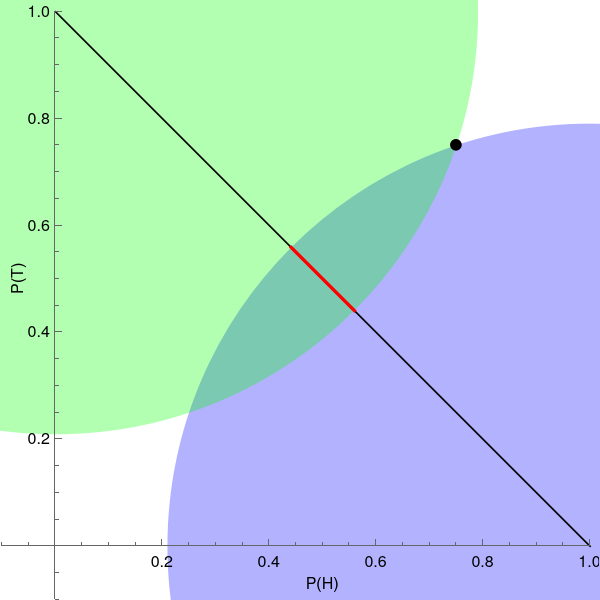
\includegraphics[width=0.7\textwidth]{Scoring rule graph.png}
\medskip
\caption{An illustration of the accuracy argument for a simple two-event $\Omega$}
\label{f:scoringrule}
\end{figure}

The claim of the scoring rule argument is that there is another probability assignment that will do better no matter what the world is.  So, what are they?  

First, let's consider what happens if the coin comes up Heads.  In that case the ideal probability assignment is the point in the lower right corner, where $P(H) = 1$ and $P(T) = 0$.  So in that world, Mandy would prefer any probability assignment that is closer to that corner to the one she currently has.  All these are illustrated by the blue circle which is centered on the point in the lower right corner.

But that's just for one possible state of the world?  What about the other?  What if the coin had come up Tails?  Now the ideal probability distribution is one where $P(H) = 0$ and $P(T) = 1$, the point in the upper left corner of our graph.  Now Mandy would prefer any probability assignment which lies within the green circle that is centered in the upper left.

Notice something about our circles: there is a lens shaped region where the two circles overlap.  Any probability assignment that lies in that region will do better {\it no matter what the state of the world is}.  Of particular interest is the part of the black line that is highlighted in red.  Those are probability assignments which are consistent with the axioms and do better than Mandy no matter what is the state of the world.

What we've shown so far is that Mandy would do better to choose any point within the lens, which includes some points that are consistent with the axioms (but also some points that are not).  What if Mandy decided to choose a point in the lens, but one that is off the line---one that is not consistent with the axioms?

We could run the same argument again (and again) until she eventually chooses a point that lies on the line. Once there, no lens-shaped region exists.  The two circles will intersect at only one point, the point that represents Mandy's probabilities.  And this fact is our theorem.  If Mandy chooses any point off the line, then there will be a lens-shaped region where she could have done better no matter what.  If Mandy chooses any point on the line, then there will not be such a region. 

Before leaving this discussion, I should take a moment to talk about why we choose the Brier score as opposed to any other way of measuring distance.  There is a long (and sometimes complicated) literature about what conditions we might want a measure of ``inaccuracy'' to obey. Many scholars argue that any inaccuracy score should be whats called a {\it proper} scoring rule.  A proper scoring rule is one that is ``self endorsing'' that is the score always regards itself as most accurate {\it when it obeys the axioms}.  Brier score is one such rule but there are others.  Space will prevent a discussion of these reasons, but interested students should look more into the literature.

\section{Descriptive concerns}

\marginnote{This study is reported in \fullcite{rottenstreich1997}.}

In a famous experiment on probability estimation, a group of US undergraduate students where asked a series of questions about the probabilities of outcomes in the next presidential election.  We can think of the underlying space as being divided into three atomic events, which we assume are exhaustive. $D$: A democrat wins the election. $R$: A republican wins the election. And $I$: an Independent (defined as neither a democrat or a republican) wins the election.  In this case $\Omega = \{D, R, I\}$. From this we might construct an additional event (so that we can test the finite activity axiom).  That event is the event $N$: ``the person who wins is not a democrat'' or $N = \{R, I\}$.

The students were divided into several groups.  Some asked to evaluate the probability of $R$, some others the probability of $I$, and some others the probability of $N$.  It turns out that in this experiment the average estimates where $P(R) = 0.59$, $P(I) = 0.05$, and $P(N) = 0.6$.  This obviously violates the axiom of additivity (assuming that we treat each group like a single individual).

The hypothesis put forward is that presentation matters. When people are asked ``will someone who is not a democrat win?'' They think of the most likely alternative, in this case a republican.  This is why $P(N) \approx P(R)$.  They forget to include the probability of an unlikely, but possible, alternative.


Another example requires just a tiny bit more work, but is regarded as more definitive.  I will give you the original example, although at this point it feels dated.  (The original is from the early 1980s.)  Subject where asked to read this brief description of ``Linda'' 

\marginnote{This study is reported in \fullcite{tversky1983}.}

\begin{quote}
Linda is 31 years old, single, outspoken and very bright. She majored in philosophy. As a student, she was deeply concerned with issues of discrimination and social justice, and also participated in anti-nuclear demonstrations.
\end{quote}

They were then asked to rank order a series of statements by how likely they were:

\begin{enumerate}
\item Linda is a teacher in elementary school. 
\item Linda works in a bookstore and takes Yoga classes. 
\item Linda is active in the feminist movement. 
\item Linda is a psychiatric social worker. 
\item Linda is a member of the League of Women Voters. 
\item Linda is a bank teller. (We will call this: $T$) 
\item Linda is an insurance salesperson. 
\item Linda is a bank teller and is active in the feminist movement. (We will call this: $A$)
\end{enumerate}

Of particular interest to the experimenters were the labeled sentences ($T$ and $A$; the labels are for our purposes and were not shown to the subjects).  They found that 85\% of their subjects ranked $A$ as more likely than $T$.  Which is impossible. 

How does this violate additivity? Here we need to be a little careful.  When defining our universe of possibilities we need to think of all the relevant ones.  If we are just concerned with whether Linda is a bank teller (or not) and whether she is a feminist (or not), then we have to consider four possibilities: 

\begin{itemize}
\item[$A$:] Linda is a feminist and a bank teller
\item[$B$:] Linda is a feminist but not a bank teller
\item[$C$:] Linda is not a feminist but is a bank teller
\item[$D$:] Linda is neither a feminist nor a bank teller
\end{itemize}

So our universe, $\Omega = \{A, B, C, D\}$.  And now we can define an event ``Linda is a bank teller'', $T = \{A, C\}$. Finite additivity requires that $P(T) = P(A) + P(C)$.  So if people say that $P(A) > P(T)$, then they are {\it either} violating finite additivity {\it or} they think that $P(C)$ is negative.  The experimenters (and me) think it's more likely that they are violating additivity than they think probabilities can be negative.  

\section{Conclusion}

This chapter has introduced probability as the way to think about uncertainty. We introduced different interpretations of probability and discussed why the axioms might be regarded as normatively compelling under those different interpretations. We concluded with two short examples that suggest that people don't always obey the axioms when evaluating the likelihood of events.

To make our lives simple, I have tended to focus on easy to understand examples (like with dice).  One might think that the axioms are (descriptively or normatively) correct for simple things that like, but be skeptical in more complex cases. Do I need to obey the axioms when evaluating the probability that Linda is a bank teller? Or that there will be a war in the next decade? Or that intelligent life exists on another planet? Etc.

Other theories with both normative and descriptive interpretations have been developed to deal with different cases.  If you're interested, I would encourage you to follow up.